\section{Математическая модель}

    В данном разделе представленно описание модели частотного скана 
    в математических выражениях.

    Согласно обзору \cite{istratov_exp_analysis} зависимость значения
    ёмкости от времени $f(t)$ для моноэкспоненциального сигнала релаксации
    имеет вид выражения \ref{eq:monoexp}.
    \begin{equation}
        \label{eq:monoexp}
        f(t) = A \exp \left(-\lambda t\right) ,
    \end{equation}
    где
    \begin{description}
        \item[\(A\)] -- амплитуда сигнала релаксации ёмкости;
        \item[\(\tau\)] -- постоянная веремени сигнала релаксации.
    \end{description}
    Спектр моноэкспоненциального сигнала релаксации имеет вид, 
    представленный на рисунке \ref{pic:monoexp_spect_example}
    \begin{figure}[ht]
        \centering
        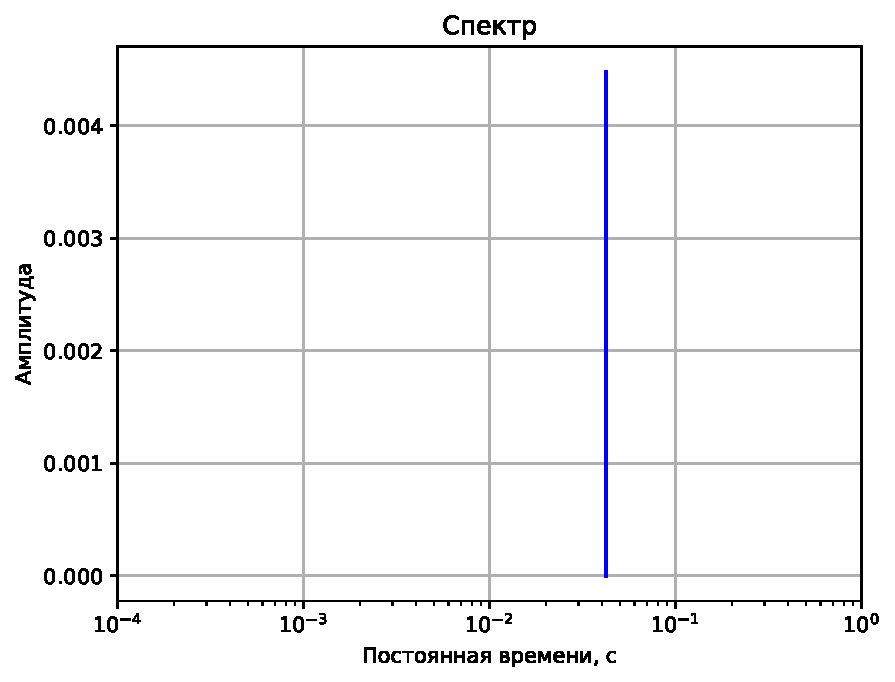
\includegraphics[width=0.75\textwidth]{monoexp_spect_expample}
        \caption{Пример спектра моноэкспоненциального сигнала релаксации
        ёмкости}
        \label{pic:monoexp_spect_example}
    \end{figure}

    Согласно \cite{istratov_exp_analysis} зависимость сигнала релаксации
    ёмкости от времени $f(t)$ для сгинала, образованного несколькими
    дискретными экспоненциальными сигналами, определяется выражением 
    \ref{eq:discr_multiexp}.
    \begin{equation}
        \label{eq:discr_multiexp}
        f(t) = \sum_{i=1}^{n}A_i\exp\left(-\lambda_i t\right) ,
    \end{equation}
    где $n$ -- количество экспоненциальных составляющих в спектре.
    Пример спектра такого сигнала показан на рисунке 
    \ref{pic:multiexp_spect_example}.
    \begin{figure}[ht]
        \centering
        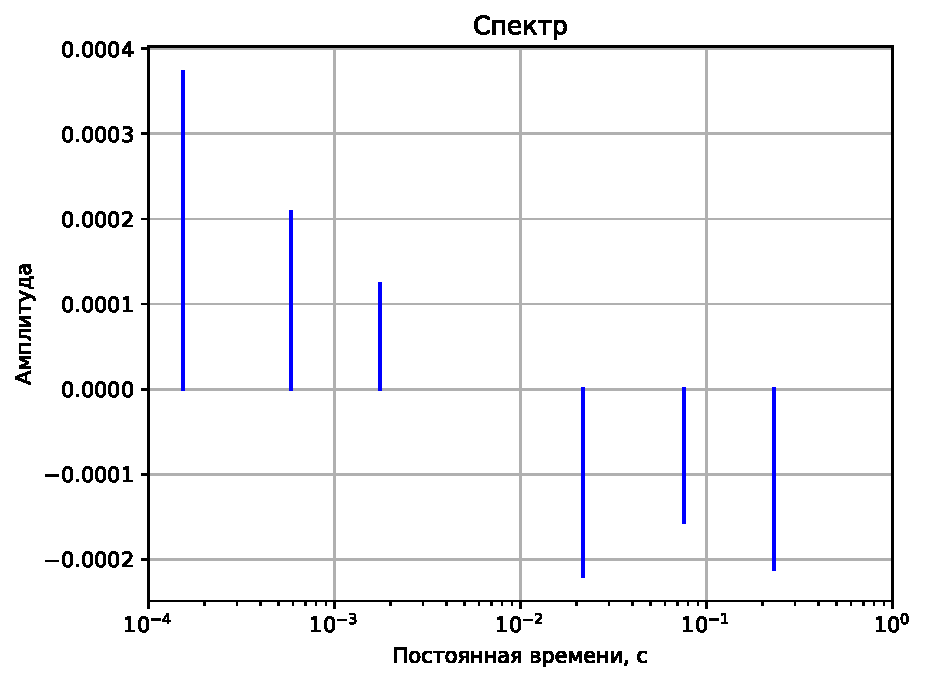
\includegraphics[width=0.75\textwidth]{multiexp_spect_example}
        \caption{Пример спектра сигнала релаксации ёмкости}
        \label{pic:multiexp_spect_example}
    \end{figure}